\documentclass{beamer}
\usetheme{Boadilla}

% Additional packages
\usepackage{graphicx}
\usepackage{amsmath}
\usepackage{booktabs}
\usepackage{hyperref}
\usepackage{natbib}
\usepackage{multirow}
\newcommand{\lowrank}{Natural GaLore}

\AtBeginSection[]{
  \begin{frame}
  \vfill
  \centering
  \begin{beamercolorbox}[sep=8pt,center,shadow=true,rounded=true]{title}
    \usebeamerfont{title}\insertsectionhead\par%
  \end{beamercolorbox}
  \vfill
  \end{frame}
}

\title{Natural GaLore: A Memory Efficient Approach for LLM Training and Finetuning}
\author{Arijit Das}
\date{\today}

\begin{document}

\begin{frame}
    \titlepage
\end{frame}

\begin{frame}{Outline}
    \tableofcontents
\end{frame}

% TODO: Change the slide footer to show the section and subsection titles
% Part 1: Set clear context and define the problem
\section{Introduction}

\begin{frame}{AI Systems}
    \begin{itemize}
        \item \textbf{Large Language Models (LLMs)} have achieved remarkable performance in various disciplines.
        \item However, turning LLMs into reliable AI systems remains challenging.
        \item Every AI system will make mistakes, but the monolithic nature of LLMs makes it difficult to understand and correct these errors.
        \item By building modular programs, using LLMs as specialized components, we can create more reliable and interpretable systems.
    \end{itemize}
\end{frame}

\begin{frame}{LLM Program}
    \begin{itemize}
        \item A LLM program \(\Phi: \mathcal{X} \to \mathcal{Y}\), is a function where input and output space \(\mathcal{X}, \mathcal{Y}\) is natural language.
        \item \(\Phi\) is assumed to make calls to modules \(\mathcal{M} = \left(\mathcal{M}_1, \mathcal{M}_2, \ldots, \mathcal{M}_{|\mathcal{M}|}\right)\) where each module \(\mathcal{M}_i: \mathcal{X}_i \to \mathcal{Y}_i\) is a declarative LLM invocation, defined via inherently fuzzy natural language descriptions.
    \end{itemize}
\end{frame}

\begin{frame}{LLM Program Optimization}
    \begin{itemize}
        \item The LLM program optimization problem is then defined by: 
            \[
            \arg \min_{\Pi, \Theta} \sum_{\left(x,y\right)\in \left(\mathcal{X} \times \mathcal{Y}\right)}\mathcal{L}(\Phi_{\Theta, \Pi}(x), y)
            \]
            given a labeled dataset \(\left(\mathcal{X} \times \mathcal{Y}\right)\) and a loss function \(\mathcal{L}\).
        \item For each module \(\mathcal{M}_i\), the optimization problem determines:
            \begin{itemize}
                \item \textbf{Prompt Optimization}: String prompt \(\Pi_i\) in which inputs \(\mathcal{X}_i\) are plugged in.
                \item \textbf{Parameter Optimization}: Weights \(\Theta_i\) which are assigned to the module \(\mathcal{M}_i\).
            \end{itemize}
    \end{itemize}
\end{frame}

\begin{frame}{LLM Program Optimization}
    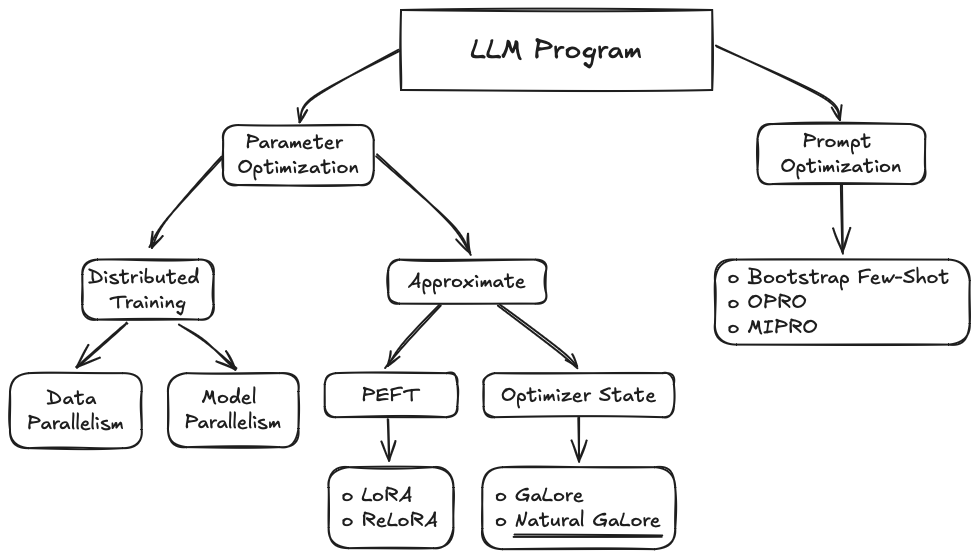
\includegraphics[width=\textwidth]{figures/LLM Program Optimization.png}
    \begin{itemize}
        \item In this work, I focus on the parameter optimization problem
    \end{itemize}
\end{frame}

% Part 2: Describe the options considered for solving the problem
\section{Parameter Optimization}

\begin{frame}{Next Token Prediction in LLMs}
    Generative LLMs predict the next token based on previously observed tokens (causal prediction).
    \begin{equation}
        \text{Prob}_{\mathbf{\theta}}(x) = \prod_{t=1}^{T} \text{Prob}_{\mathbf{\theta}}(x_t \mid x_{<t})
    \end{equation}
    where \( x_{<t} = (x_1, x_2, \dots, x_{t-1}) \).
\end{frame}

\begin{frame}{Objective: Negative Log-Likelihood (NLL)}
    \begin{itemize}
        \item The training objective is to minimize the Negative Log-Likelihood (NLL):
    \end{itemize}
    \begin{equation}
        \Phi(\mathbf{\theta}) = -\sum_{t=1}^{T} \log \text{Prob}_{\mathbf{\theta}}(x_t \mid x_{<t})
        \label{eq:cross_entropy_loss}
    \end{equation}
    \begin{itemize}
        \item Penalizes low probability assignments to correct tokens.
        \item High-dimensional, non-convex optimization problem.
    \end{itemize}
\end{frame}

\begin{frame}{Parameter Optimization}
    \begin{itemize}
        \item Training and fine-tuning LLMs demand enormous computational resources and are highly memory-intensive.
        \item Memory requirements: 
        \begin{itemize}
            \item Stem from storing billions of parameters, gradients, and optimizer states.
            \item For example pre-training a Llama-7B model, just the model requires 72GB of memory: 14GB for parameters and gradients each, 42GB for optimizer states and 2GB for activations. 
            \item Limit the ability to train large models on hardware with limited memory capacity.
            \item Increase training costs and environmental impact.
        \end{itemize}
        \item \textbf{Objective}: Develop a memory-efficient approach for training and fine-tuning LLMs without sacrificing performance.
    \end{itemize}
\end{frame}

\begin{frame}{Distributed Training Techniques}
    \begin{itemize}
        \item \textbf{Data Parallelism}
            \begin{itemize}
                \item DDP combines data parallelism with efficient gradient synchronization.
                \item \textbf{Pros}: Efficient gradient updates, good scalability.
                \item \textbf{Cons}: Memory bottlenecks persist when model size exceeds single GPU capacity.
            \end{itemize}
        \item \textbf{Model Parallelism}
            \begin{itemize}
                \item Partitions model across multiple devices.
                \item Techniques: Pipeline parallelism \citep{huangGPipeEfficientTraining2019}, Tensor parallelism \citep{shoeybiMegatronLMTuningScaling2019}, Fully Sharded Data Parallel (FSDP) \citep{zhaoExtendingTorchElasticStateful2020}.
                \item \textbf{Pros}: Allows training of models larger than a single GPU.
                \item \textbf{Cons}: Communication overhead, complex implementation.
            \end{itemize}
    \end{itemize}
\end{frame}

\begin{frame}{Distributed Training Techniques}
    \begin{itemize}
        \item Data and Model Parallelism can be augmented with further techniques to reduce memory usage.
        \item \textbf{Gradient Checkpointing} \citep{chenTrainingDeepNets2016}
            \begin{itemize}
                \item Stores subset of activations during forward pass.
                \item Recomputes activations during backward pass.
                \item \textbf{Pros}: Reduces memory usage.
                \item \textbf{Cons}: Increases computational overhead.
            \end{itemize}
        \item \textbf{Memory Offloading}
            \begin{itemize}
                \item Moves optimizer states and gradients to CPU memory.
                \item Techniques: ZeRO-Offload \citep{rajbhandariZeROMemoryOptimizations2020}.
                \item \textbf{Pros}: Significant memory reduction.
                \item \textbf{Cons}: Increased system complexity, operational costs.
            \end{itemize}
    \end{itemize}
\end{frame}

\begin{frame}{Parameter-Efficient Fine-Tuning (PEFT)}
    \begin{itemize}
        \item \textbf{LoRA (Low-Rank Adaptation)} \citep{huLoRALowRankAdaptation2021}
            \begin{itemize}
                \item Reparameterizes weight matrices using low-rank adapters
                \begin{equation}
                    W = W_0 + BA, \quad B \in \mathbb{R}^{n \times r}, A \in \mathbb{R}^{r \times m}
                \end{equation}
                \item \textbf{Pros}: Reduces trainable parameters, lowers memory usage
                \item \textbf{Cons}: May not match full fine-tuning performance, especially on complex tasks \citep{xiaChainLoRAEfficient2024}.
            \end{itemize}
        \item \textbf{ReLoRA} \citep{lialinReLoRAHighRankTraining2023}
            \begin{itemize}
                \item Extends LoRA for pre-training.
                \item Periodically updates frozen weights using learned adapters.
                \item \textbf{Pros}: Enables continual learning with lower memory.
                \item \textbf{Cons}: Requires initial full-rank training phase.
            \end{itemize}
    \end{itemize}
\end{frame}

\begin{frame}{GaLore: Gradient Low-Rank Approximation}
    \begin{itemize}
        \item Exploits low-rank structure of gradients to approximate optimizer states \citep{zhao2024galore}.
        \item Projects gradients \(\mathbf{g} \in \mathbb{R}^{n \times m}\) into a low-rank form using Singular Value Decomposition: \(\mathbf{g} = \mathbf{P} \Sigma \mathbf{Q}^{T}\)
        \begin{equation}
            \mathbf{g}_{\text{low-rank}} = \mathbf{P}^{T} \mathbf{g}, \quad \mathbf{P} \in \mathbb{R}^{n \times r}
        \end{equation}
        \item \textbf{Pros}:
            \begin{itemize}
                \item Significant memory reduction (up to 30\% compared to LoRA).
                \item Full-parameter updates, maintaining model capacity.
            \end{itemize}
        \item \textbf{Cons}:
            \begin{itemize}
                \item Performance may not match full optimizer state methods.
                \item Low-rank approximation may not capture full optimization dynamics.
            \end{itemize}
    \end{itemize}
\end{frame}

% Part 3: Describe the proposed approach
\section{Proposed Approach}

\begin{frame}{Natural GaLore: Our Approach}
    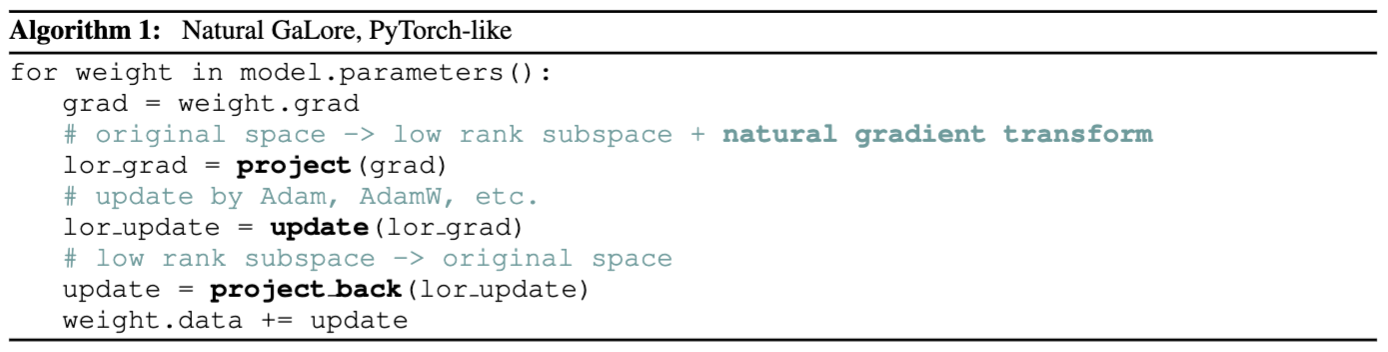
\includegraphics[width=\textwidth]{figures/natural_galore_algorithm.png}
    \begin{itemize}
        \item \textbf{Goal}: Accelerating convergence of GaLore to bridge the gap with AdamW.
        \item \textbf{Key Idea}: Incorporate second-order information using the Fisher Information Matrix (FIM) to estimate natural gradients.
    \end{itemize}
\end{frame}

\subsection{Low-Rank Gradient Descent}

\begin{frame}{Low-Rank Gradient Descent in GaLore}
    \begin{itemize}
        \item GaLore restricts updates to an affine subspace:
    \end{itemize}
    \begin{equation}
        \mathbf{u}_k \in \mathbf{\theta}_k + \text{Range}(\mathbf{P}_k)
    \end{equation}
    \begin{itemize}
        \item Projection matrix \(\mathbf{P}_k \in \mathbb{R}^{n \times r}\) computed using compact SVD of the gradient matrix.
    \end{itemize}
\end{frame}

\begin{frame}{Taylor Series Approximation of Loss}
    \begin{equation}
        \Phi(\mathbf{\theta}_k + \mathbf{P}_k \mathbf{u}_k) \approx \Phi(\mathbf{\theta}_k) + \mathbf{g}_k^T \mathbf{u}_k + \frac{1}{2} \mathbf{u}_k^T \mathbf{H}_k \mathbf{u}_k
        \label{eq:taylor_series_expansion}
    \end{equation}
    where:
    \begin{itemize}
        \item \(\mathbf{g}_k = \mathbf{P}_k^T \nabla_{\mathbf{\theta}} \Phi(\mathbf{\theta}_k)\) is the projected gradient.
        \item \(\mathbf{H}_k = \mathbf{P}_k^T \nabla^2_{\mathbf{\theta}} \Phi(\mathbf{\theta}_k) \mathbf{P}_k\) is the local Hessian matrix.
    \end{itemize}
\end{frame}

\begin{frame}{Fisher Information Matrix (FIM) Approximation}
    \begin{equation}
        \mathbf{F}_k = \mathbb{E}_{x \sim p_{\text{data}}} [ \mathbf{H}_k ]
    \end{equation}
    \begin{itemize}
        \item The FIM captures the curvature of the loss landscape.
        \item Empirically estimated by:
    \end{itemize}
    \begin{equation}
        \mathbf{\hat{F}}_k = \frac{1}{h} \sum_{k=1}^{h} \mathbf{g}_k \mathbf{g}_k^T
    \end{equation}
\end{frame}

\begin{frame}{Optimal Update Direction}
    \begin{equation}
        \mathbf{u}_k^* = \mathbf{\hat{F}}_k^{-1} \mathbf{g}_k
        \label{eq:optimal_direction}
    \end{equation}
    \begin{itemize}
        \item Minimizes the loss in the local neighborhood.
        \item Leads to the following update step:
    \end{itemize}
    \begin{equation}
        \mathbf{\theta}_{k+1} = \mathbf{\theta}_k - \eta \mathbf{P}_k \mathbf{u}_k^*
        \label{eq:gradient_descent_update}
    \end{equation}
\end{frame}

\subsection{LowRank and Fisher Efficiency}

\begin{frame}{Improving GaLore with Fisher Efficiency}
    \begin{itemize}
        \item GaLore’s performance can be improved by incorporating second-order information via FIM.
        \item Natural gradient descent is Fisher efficient and reduces variance in gradient updates.
    \end{itemize}
    \begin{equation}
        \text{Var}[\mathbf{\theta}_k] = \frac{1}{mk} \mathbf{F}_k^{-1}(\mathbf{\theta}_k^*) + \mathcal{O}\left(\frac{1}{k^2}\right)
        \label{eq:variance_reduction}
    \end{equation}
    \begin{itemize}
        \item Smaller variance translates to faster convergence.
    \end{itemize}
\end{frame}

\subsection{Natural Gradient Transform}

\begin{frame}{Woodbury Identity for Efficient Natural Gradient}
    \begin{equation}
        (A + UBU^T)^{-1} = A^{-1} - A^{-1}U(B^{-1} + U^TA^{-1}U)^{-1}U^TA^{-1}
    \end{equation}
    \begin{itemize}
        \item Used to compute the inverse FIM efficiently.
        \item Allows memory-efficient computation of the natural gradient.
    \end{itemize}
\end{frame}

\begin{frame}{Natural Gradient Estimate}
    \begin{equation}
        \mathbf{\tilde{g}}_k = \frac{1}{\lambda}\mathbf{g}_k - \frac{1}{\lambda} G (\lambda I + G^T G)^{-1} G^T \mathbf{g}_k
    \end{equation}
    where:
    \begin{itemize}
        \item \(G = [\operatorname{vec}(\mathbf{g}_k), \ldots, \operatorname{vec}(\mathbf{g}_{k-s})]\) is the gradient history.
    \end{itemize}
\end{frame}

\begin{frame}{Efficient Computation with Cholesky Decomposition}
    \begin{equation}
        S z = y, \quad S = I + \frac{1}{\lambda} G^T G
    \end{equation}
    \begin{itemize}
        \item Solved using Cholesky decomposition to compute the natural gradient in \(\mathcal{O}(s^2)\) time.
        \item Enables scalable low-rank optimization.
    \end{itemize}
\end{frame}

\begin{frame}{Conclusion: Memory-Efficient Second-Order Optimization}
    \begin{itemize}
        \item Natural GaLore combines low-rank projection with efficient second-order updates.
        \item Improves convergence and reduces memory consumption.
        \item Fisher efficiency allows faster optimization in high-dimensional, non-convex spaces.
    \end{itemize}
\end{frame}

\begin{frame}{Natural Gradient Transform}
    \begin{itemize}
        \item \textbf{Method}:
            \begin{itemize}
                \item Apply inverse FIM to low-rank gradients from GaLore.
                \item Utilize Woodbury Identity and Cholesky Decomposition for efficient computation.
            \end{itemize}
        \item \textbf{Benefits}:
            \begin{itemize}
                \item Faster convergence.
                \item Variance reduction in gradient estimates.
                \item Better utilization of curvature information.
            \end{itemize}
    \end{itemize}
\end{frame}

\begin{frame}{Natural Gradient Computation}
    \begin{itemize}
        \item \textbf{Optimal Update Direction}:
            \[
            \mathbf{u}_k^* = \mathbf{\hat{F}}_k^{-1} \mathbf{g}_k
            \]
            where \(\mathbf{\hat{F}}_k\) is the empirical Fisher Information Matrix.
        \item \textbf{Parameter Update}:
            \[
            \mathbf{\theta}_{k+1} = \mathbf{\theta}_k - \eta \mathbf{P}_k \mathbf{u}_k^*
            \]
        \item \textbf{Efficient Inverse FIM Computation}:
            \begin{itemize}
                \item Use Woodbury Identity:
                    \[
                    (\lambda I + GG^T)^{-1} = \frac{1}{\lambda} I - \frac{1}{\lambda^2} G (I + \frac{1}{\lambda} G^T G)^{-1} G^T
                    \]
                \item Compute using Cholesky Decomposition and matrix-vector products.
            \end{itemize}
    \end{itemize}
\end{frame}

\begin{frame}{Advantages of Our Approach}
    \begin{itemize}
        \item \textbf{Incorporates Curvature Information}:
            \begin{itemize}
                \item Accounts for the geometry of the loss landscape.
                \item Enables more informed optimization steps.
            \end{itemize}
        \item \textbf{Variance Reduction}:
            \begin{itemize}
                \item Reduces variance in gradient estimates.
                \item Leads to faster convergence, especially in limited iterations.
            \end{itemize}
        \item \textbf{Memory Efficiency}:
            \begin{itemize}
                \item Maintains low memory footprint.
                \item Can be implemented without significant computational overhead.
            \end{itemize}
    \end{itemize}
\end{frame}

% Part 4: Experiments and Results
\section{Experiments and Results}

\begin{frame}{Pre-training Experiments on C4 Dataset}
    \begin{itemize}
        \item \textbf{Models}: LLaMA variants with 60M, 300M, and 1.1B parameters.
        \item \textbf{Dataset}: C4 dataset.
        \item \textbf{Metrics}: Validation perplexity, memory consumption.
        \item \textbf{Results}:
            \begin{itemize}
                \item Our method achieves lower perplexity than GaLore across all model sizes.
                \item Closer performance to full optimizer state methods.
                \item Maintains significant memory savings.
            \end{itemize}
        \item \textbf{Conclusion}: Incorporating natural gradients enhances performance without additional memory overhead.
    \end{itemize}
\end{frame}

\begin{frame}{Pre-training Experiments on C4 Dataset}
    \begin{table}[ht]
        \centering
        \caption{\small{Comparison of \textit{\lowrank} with other low-rank algorithms on pre-training various sizes of LLaMA models on the C4 dataset. Validation log perplexity is reported (averaged over 5 runs), along with a memory estimate (in gigabytes) of the total parameters and optimizer states based on BF16 format.}}
        \label{tab:lora_compare_llama}
        \resizebox{\linewidth}{!}{\begin{tabular}{lcccc}
        \toprule
                         & \textbf{60M} & \textbf{130M} & \textbf{350M} & \textbf{1.1B} \\
        \midrule
        Full-Rank        & 3.52 (0.36G) & 3.22 (0.76G) & 2.93 (2.06G) & 2.72 (7.80G) \\
        \midrule
        \textit{\lowrank} & \textbf{3.53} (0.24G) & \textbf{3.22} (0.52G) & \textbf{2.93} (1.22G) & \textbf{2.80} (4.38G) \\
        GaLore           & 3.56 (0.24G) & 3.24 (0.52G) & 2.95 (1.22G) & 2.90 (4.38G) \\
        Low-Rank         & 4.35 (0.26G) & 3.82 (0.54G) & 3.62 (1.08G) & 4.96 (3.57G) \\
        LoRA             & 3.55 (0.36G) & 3.52 (0.80G) & 3.24 (1.76G) & 2.96 (6.17G) \\
        ReLoRA           & 3.61 (0.36G) & 3.38 (0.80G) & 3.37 (1.76G) & 2.91 (6.17G) \\
        \bottomrule
        Rank $r / d_{\text{model}}$ & 128 / 256 & 256 / 768 & 256 / 1024 & 512 / 2048 \\
        Training Tokens  & 1.1B & 2.2B & 6.4B & 13.1B \\
        \bottomrule
        \end{tabular}}
    \end{table}
\end{frame}

\begin{frame}{Fine-Tuning on GLUE Benchmark}
    \begin{itemize}
        \item \textbf{Model}: RoBERTa-Base.
        \item \textbf{Benchmark}: GLUE tasks (CoLA, MRPC, STS-B, etc.).
        \item \textbf{Comparison} with LoRA and full fine-tuning.
        \item \textbf{Results}:
            \begin{itemize}
                \item Comparable or better performance than LoRA.
                \item Achieved an average score of 86.05, close to full fine-tuning baseline of 86.28.
                \item Less memory consumption.
            \end{itemize}
        \item \textbf{Conclusion}: Effective for memory-efficient fine-tuning without sacrificing accuracy.
    \end{itemize}
\end{frame}

\begin{frame}{Fine-Tuning on GLUE Benchmark}
    \begin{table}[ht]
        \caption{\small{Evaluating \textit{\lowrank} for memory-efficient fine-tuning on the GLUE benchmark using pre-trained RoBERTa-Base. We report the average score of all tasks. Memory consumption is reported in millions of parameters (M).}}
        \label{tab:fine_tuning}
        \centering
        \resizebox{\linewidth}{!}{%
        \begin{tabular}{l|c|cccccccc|c}
        \toprule
                   & \textbf{Memory} & \textbf{CoLA} & \textbf{STS-B} & \textbf{MRPC} & \textbf{RTE} & \textbf{SST-2} & \textbf{MNLI} & \textbf{QNLI} & \textbf{QQP} & \textbf{Avg} \\
        \midrule
        Full Fine-Tuning & 747M & 62.24 & 90.92 & 91.30 & 79.42 & 94.57 & 87.18 & 92.33 & 92.28 & 86.28 \\
        \midrule
        \textbf{\textit{\lowrank} (rank=4)} & 253M & 61.50 & \textbf{90.80} & \textbf{92.10} & \textbf{79.50} & \textbf{94.20} & \textbf{87.05} & \textbf{92.30} & 91.15 & \textbf{86.05} \\
        GaLore (rank=4) & 253M & 60.35 & 90.73 & 92.25 & 79.42 & 94.04 & 87.00 & 92.24 & 91.06 & 85.89 \\
        LoRA (rank=4) & 257M & \textbf{61.38} & 90.57 & 91.07 & 78.70  & 92.89 & 86.82 & 92.18 & \textbf{91.29} & 85.61 \\
        \midrule
        \textbf{\textit{\lowrank} (rank=8)} & 257M & 61.70 & \textbf{90.90} & \textbf{92.25} & \textbf{79.80} & \textbf{94.40} & \textbf{87.20} & \textbf{92.35} & \textbf{91.25} & \textbf{86.23} \\
        GaLore (rank=8) & 257M & 60.06 & 90.82 & 92.01 & 79.78 & 94.38 & 87.17 & 92.20 & 91.11 & 85.94 \\
        LoRA (rank=8) & 264M & \textbf{61.83} & 90.80 & 91.90 & 79.06  & 93.46 & 86.94 & 92.25 & 91.22 & 85.93 \\
        \bottomrule
        \end{tabular}
        }
        \vskip -0.1in
    \end{table}
\end{frame}

\begin{frame}{Fine-Tuning for Function Calling in AAS}
    \begin{itemize}
        \item \textbf{Task}: Function calling using TinyAgent framework.
        \item \textbf{Model}: TinyLlama 1.1B.
        \item \textbf{Dataset}: TinyAgent dataset with 40K examples.
        \item \textbf{Metrics}: Success rate in generating correct function-calling plans.
        \item \textbf{Results}:
            \begin{itemize}
                \item Our method achieves a success rate of \textbf{83.09\%}.
                \item Outperforms 16-bit LoRA (80.06\%) and GPT-4-turbo by 4\%.
                \item Uses \textbf{30\% less memory}.
            \end{itemize}
        \item \textbf{Conclusion}: Enhances performance of smaller models, making them competitive with larger models.
    \end{itemize}
\end{frame}

\begin{frame}{Fine-Tuning for Function Calling in AAS}
    \begin{table}[ht]
        \vspace{-3mm}
        \caption{
        Latency, size, and success rate of TinyAgent models before and after quantization. Latency is the end-to-end latency of the function calling planner, including the prompt processing time and generation.}
        \label{table:t2}
        \centering
        \resizebox{\linewidth}{!}{%
        \begin{tabular}{c|c|c|c|c}
            \toprule
            Model &	Weight Precision &	Latency (seconds)	& Model Size (GB)	& Success Rate (\%) \\
            \midrule
            GPT-3.5 & Unknown & 3.2 & Unknown & 65.04 \\
            GPT-4-Turbo & Unknown & 3.9 & Unknown & 79.08 \\
            \midrule
            \multirow{2}{*}{TinyAgent-1.1B} & 16-bit (\textit{\lowrank}) & 3.9 & 2.2 & \textbf{83.09} \\
            & 16-bit (LoRA) & 3.9 & 2.2 & 80.06 \\
            \midrule
            \multirow{1}{*}{TinyAgent-7B} & 16-bit \citep{erdogan2024tinyagent} & 19.5 & 14.5 & 84.95 \\
            \bottomrule
            \end{tabular}
        }
        \vskip -0.1in
    \end{table}
\end{frame}

% Part 5: Conclusion
\section{Conclusion}

\begin{frame}{Conclusion}
    \begin{itemize}
        \item Presented \textbf{Natural GaLore}, a memory-efficient approach for LLM training and fine-tuning.
        \item Enhanced GaLore by incorporating \textbf{natural gradients} for better performance.
        \item Achieved significant memory savings without sacrificing accuracy.
        \item Validated effectiveness through extensive experiments on pre-training and fine-tuning tasks.
        \item Demonstrated practical benefits in advanced agentic systems.
    \end{itemize}
\end{frame}

\begin{frame}{Future Work}
    \begin{itemize}
        \item Explore \textbf{low-memory and structured projection matrices} for further memory efficiency.
        \item Conduct more extensive empirical evaluations on fine-tuning tasks in Advanced Agentic Systems.
        \item Inspire future research on \textbf{optimizer state approximation} for memory-efficient training.
        \item Make large-scale model training more accessible on consumer-grade hardware.
    \end{itemize}
\end{frame}

\begin{frame}{Thank You}
    \begin{center}
        Questions?
    \end{center}
\end{frame}

\begin{frame}[allowframebreaks]{References}
    \small
    \bibliography{iclr_template/iclr2025_conference}
    \bibliographystyle{iclr_template/iclr2025_conference}
\end{frame}

\end{document}